\section{Approximationssatz von Stone-Weierstraß}

\begin{frame}{Funktionenalgebra}
    \begin{defi}[Funktionenalgebra]
        Eine Menge \( \mathcal{A} \subset \mathcal{C}^0(M) \) heißt 
        \textit{Funktionenalgebra}, wenn sie geschlossen unter Addition, 
        skalarer Multiplikation und Funktionenmultiplikation ist, 
        d.~h. \( \forall f,g \in \A, c \in \mathbb{R} \)
        \[ f + g \in \mathcal{A}, \quad c \cdot f \in \mathcal{A}, \quad f \cdot g \in \mathcal{A}. \]
    \end{defi}
\end{frame}

\begin{frame}{Verschwinden}
    \begin{defi}[Verschwinden]
        Eine Funktionenalgebra \(\A \subset \CM\) 
        \textit{verschwindet} an einem Punkt \(p \in M\), falls 
        \[ f(p) = 0 \;\forall f \in \mathcal{A}. \]
    \end{defi}
    \pause
    \begin{bsp}
        \( \A := \set{ x \mapsto \sum_{j=1}^n a_n x^n \;|\; n\in \N, a_j \in \R, j = 1,\ldots, n } \subset \mathcal{C}^0([-1,1]) \) 
        verschwindet im Punkt \(0\).
    \end{bsp}
\end{frame}

\begin{frame}{Punktetrennend}
    \begin{defi}
        Eine Funktionenalgebra \(\A \subset \CM\) ist \textit{punktetrennend}, 
        wenn \( \forall p_1, p_2 \in M \) eine Funktion \(f \in \A\) existiert, 
        sodass \( f(p_1) \neq f(p_2) \).
    \end{defi}
    \pause
    \begin{bsp}
        \( \A := \set{ x \mapsto \sum_{j=0}^n a_{j} x^{2j} \;|\; n\in\N, a_j \in \R, j = 1,\ldots, n } 
        \subset \mathcal{C}^0([-1,1]) \)
        trennt die Punkte \( z \) und \(-z\) (\(z \in [-1,1] \setminus \set{0} \)) nicht, da \( \forall f \in \A \) gilt 
        \( f(z) = f(-z) \).
    \end{bsp}
    \pause
    \begin{bsp}
        Die Funktionenalgebra aller trigonometrischen Polynome auf \( [0,2\pi) \) 
        separiert Punkte und verschwindet nirgends.
    \end{bsp}
\end{frame}

\begin{frame}{Satz von Stone-Weierstraß}
    \begin{satz}[Satz von Stone-Weierstraß]
        Sei \(M\) ein kompakter metrischer Raum und \( \mathcal{A} \) eine punktetrennende
        Funktionenalgebra in \( \mathcal{C}^0(M) \), die nirgends verschwindet. 
        Dann ist \( \mathcal{A} \) dicht in \( \mathcal{C}^0(M) \).
    \end{satz}
    \pause
    \begin{bem}
        Der Satz von Stone-Weierstraß ist offensichtlich eine Verallgemeinerung 
        des Satzes von Weierstraß. 
        Wir benötigen die Aussage des Satzes von Weierstraß für den Beweis von Stone-Weierstraß.
    \end{bem}
\end{frame}

\begin{frame}
    \begin{lem}\label{bel-punkte}
        Sei \( \A \subset \CM \) eine punktetrennende Funktionenalgebra, die nirgends verschwindet. 
        Dann existiert für beliebige \( p_1, p_2 \in M, p_1\neq p_2, 
        c_1, c_2 \in \R \)
        ein \(f \in \A\) mit 
        \[ f(p_1) = c_1, \quad f(p_2) = c_2. \]
    \end{lem}
\end{frame}

\begin{frame}{Beweis von Lemma \ref{bel-punkte}}
    Seien \( p_1, p_2 \in M \) und \( c_1, c_2 \in \R \) gegeben. 
    \pause

    Da \(\A\) nirgends verschwindet, existieren \( g_1, g_2 \in \A \), 
    sodass 
    \( g_1(p_1) \neq 0, g_2(p_2) \neq 0 \). 
    \pause

    Also gilt \( g := g_1^2 + g_2^2 \in \A \). \(g\) verschwindet weder in \(p_1\) noch \(p_2\).
    \pause 

    \(\A\) trennt Punkte, also existiert ein \( h \in \A \), sodass 
    \( h(p_1) \neq h(p_2) \).
    \pause 
    Betrachten wir die Matrix 

    \[ H = \begin{pmatrix}
        a & ab \\
        c & cd
    \end{pmatrix} = \begin{pmatrix}
        g(p_1) & g(p_1) h(p_1) \\
        g(p_2) & g(p_2) h(p_2)
    \end{pmatrix}. \]
    \pause

    Nach Konstruktion gilt 
    \( a, c \neq 0 \) sowie \(b \neq d\). Also gilt \( \det H = acd - abc = ac(d - b) \neq 0 \). 
\end{frame}

\begin{frame}
    Somit hat das LGS 
    \begin{align*}
        a \xi + ab \eta &= c_1 \\
        c \xi + cd \eta &= c_2
    \end{align*}

    genau eine Lösung für \( \xi \) und \( \eta \). 
    \pause
    Sei \( f := \xi g + \eta g h \). \pause 
    Offensichtlich ist \( f \in \A \) \pause 
    und es gilt 
    \begin{align*}
        f(p_1) &= \xi g(p_1) + \eta g(p_1) h(p_1) = c_1, \\
        f(p_2) &= \xi g(p_2) + \eta g(p_2) h(p_2) = c_2.
    \end{align*}
    \qed
\end{frame}

\begin{frame}
    \begin{lem}\label{abg-algebra}
        Sei \( \A \subset \CM \) eine Funktionenalgebra 
        sowie \(M\) ein kompakter metrischer Raum.
        Dann ist \( \Abar \) ebenfalls eine Funktionenalgebra.
    \end{lem}
    Beweis: \pause 
    Stimmt so. \qed
\end{frame}

\begin{frame}
    \begin{lem}\label{betrag-in-algebra}
        Sei \( \A \subset \CM \) eine Funktionenalgebra. Dann gilt 
        \[ f \in \Abar \Rightarrow \abs{f} \in \Abar \]
        sowie 
        \[ f_1, \ldots, f_n \in \Abar \Rightarrow \max(f_1,\ldots, f_n), \min(f_1,\ldots, f_n) \in \Abar. \]
    \end{lem} \pause
    Beweis:
    Nach dem Satz von Weierstraß existiert ein Polynom 
    \( p(y) \), sodass 
    \[ \sup \set{ \abs{ p(y) - \abs{y} } 
    \;|\; \abs{y} \leq \norm{f} } < \frac{\varepsilon}{2}, \]
    da \( \abs{y} \in \C([-\norm{f}, \norm{f}]) \). 
    \pause

    Der konstante Term dieses Polynoms ist höchstens \( \varepsilon / 2 \), 
    da \( \abs{ p(0) - \abs{0} } < \varepsilon/2 \).
\end{frame}

\begin{frame}
    Sei \( q := p - p(0) \). Dann ist \( q(y) \) ein 
    Polynom mit Konstante \(0\) und es gilt 
    \[ \abs{ q(y) - \abs{y} } < \varepsilon 
    \;\forall y \in [-\norm{f}, \norm{f}]. \]
    \pause

    Schreiben wir nun \( q \) als 
    \( q(y) = a_1 y + a_2 y^2 + \cdots + a_n y^n \) und 
    \[ g = a_1 f + a_2 f^2 + \cdots + a_n f^n. \]
    \pause

    Da \( \Abar \) eine Funktionenalgebra nach Lemma \ref{abg-algebra}
    und somit gilt 
    \( g \in \Abar \). 
    \pause

    Sei \( x\in M \) und \( y = f(x) \). Dann gilt 
    \[ \abs{ g(x) - \abs{f(x)} } = \abs{ q(y) - \abs{y} } < \varepsilon. \]
    \pause
    
    Also folgt \( \abs{f} \in \Abarbar = \Abar \). 
\end{frame}

\begin{frame}
    Außerdem gilt falls \(f,g \in \Abar \)
    \pause
    \begin{align*}
        \max(f,g) &= \frac{f+g}{2} + \frac{\abs{f-g}}{2}, \\
        \min(f,g) &= \frac{f+g}{2} - \frac{\abs{f-g}}{2}.
    \end{align*} 
    \pause
    Also gilt \( \max(f,g), \min(f,g) \in \Abar \). 
    \pause

    Mittels Wiederholung können wir dies für beliebige 
    \( f_1, \ldots, f_n \in \Abar \) fortführen.
    \qed
\end{frame}

\begin{frame}{Beweis vom Satz von Stone-Weierstraß}
    Sei \( \A \) eine punktetrennende Funktionenalgebra in \(\CM\), die nirgends verschwindet. \pause
    Wir zeigen nun, dass \( \A \) dicht in \(\CM\) ist. \pause
    D. h. für ein gegebenes \( F \in \CM, \varepsilon > 0 \) 
    müssen wir ein \( G \in \A \) finden, sodass 
    \[ F(x) - \varepsilon < G(x) < F(x) + \varepsilon. \]
    \pause

    Wir betrachten nun zwei Punkte \(p\neq q \in M\).
    Nach Lemma \ref{bel-punkte} existiert ein \(H_{pq} \in \A\), 
    sodass 
    \[ H_{pq}(p) = F(p), \quad H_{pq}(q) = F(q). \]
\end{frame}

\begin{frame}
    \begin{columns}
        \begin{column}{0.4\textwidth}
            Wir fixieren nun \(p\).
            \onslide<2->{Für jedes \(q \in M\) existiert eine Umgebung 
            \( U_q \)}\onslide<3->{, sodass 
            \[ x \in U_q \Rightarrow F(x) - \varepsilon < H_{pq}(x). \]}
            % H_{pq} ist stetig
        \end{column}
        \begin{column}{0.6\textwidth}
            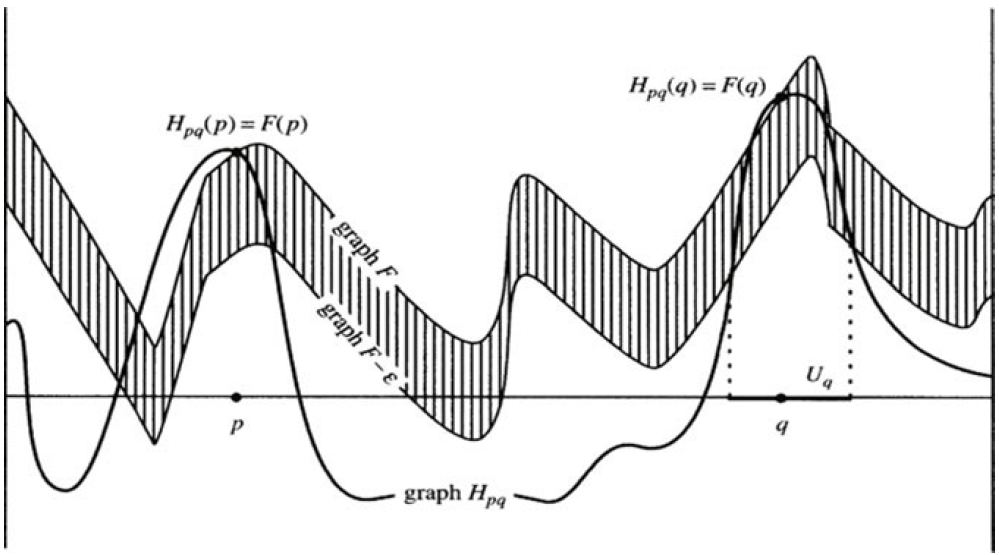
\includegraphics[width=\textwidth]{images/stone-weierstrass-step1.png}
        \end{column}
    \end{columns}
\end{frame}

\begin{frame}
    % todo Memo mit Überdeckungskompaktheit
    \begin{columns}
        \begin{column}{0.4\textwidth}
            \( M \) ist kompakt \( \Rightarrow \) endlich viele 
            \( U_{q_1}, \ldots, U_{q_n} \) überdecken \(M\).
            \onslide<2->{Sei 
            \[ G_p := \max(H_{pq_1}, \ldots, H_{pq_n}). \]}
            
            \onslide<4->{Nach Lemma \ref{betrag-in-algebra} gilt \( G_p \in \Abar \).}
            \onslide<5->{Es gilt nun \(G_p(p) = F(p)\)} \onslide<6->{sowie \( \forall x \in M \)
            \[ F(x) - \varepsilon < G_p(x). \]}
        \end{column}
        \begin{column}{0.6\textwidth}
            \onslide<3->{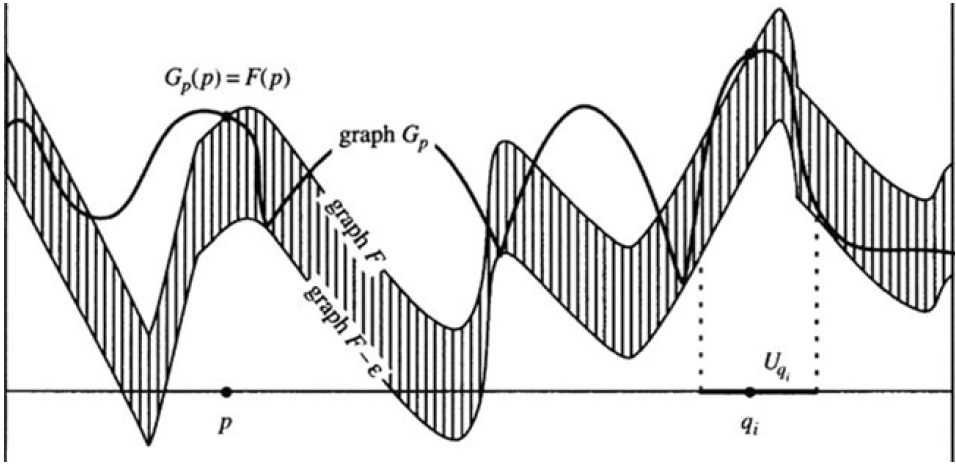
\includegraphics[width=\textwidth]{images/stone-weierstrass-step2.png}}
        \end{column}
    \end{columns}
\end{frame}

\begin{frame}
    \begin{columns}
        \begin{column}{0.4\textwidth}
            Sei nun \(p\) variabel.
            \onslide<2->{\(G_p\) stetig}
            \onslide<3->{\( \Rightarrow \forall p \in M \;\exists V_p: \)
            \[ x_p \in V_p \Rightarrow G_p(x) < F(x) + \varepsilon. \]}

            \onslide<5->{Nun folgt wieder aus der Kompaktheit von \(M\), dass 
            endlich viele \( V_{p_1}, \ldots, V_{p_m} \) \(M\) überdecken.}
        \end{column}
        \begin{column}{0.6\textwidth}
            \onslide<4->{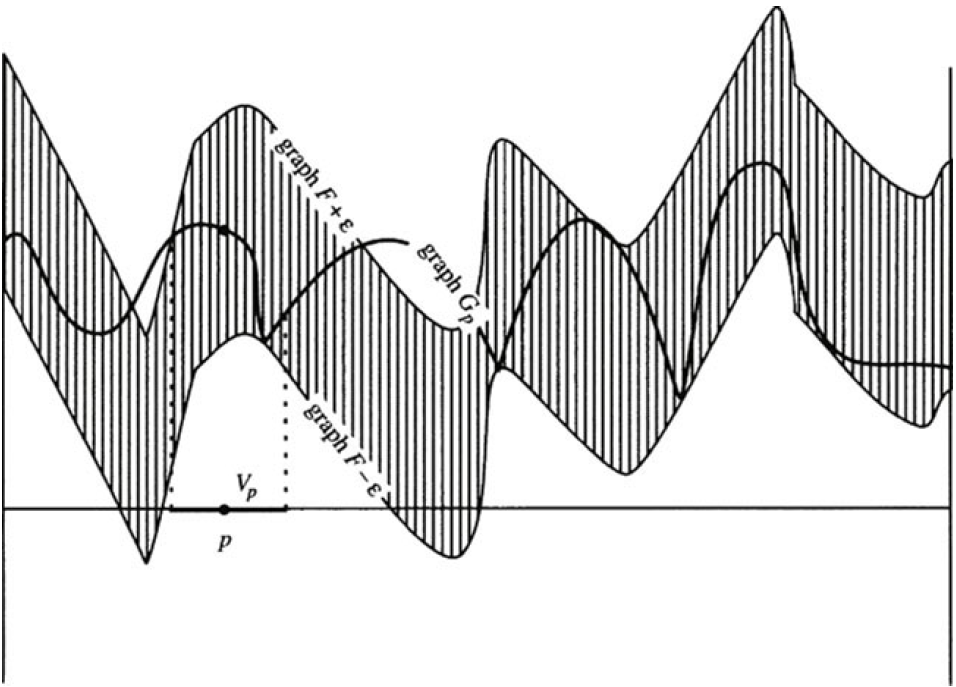
\includegraphics[width=\textwidth]{images/stone-weierstrass-step3.png}}
        \end{column}
    \end{columns}
\end{frame}

\begin{frame}
    \begin{columns}
        \begin{column}{0.4\textwidth}
            Sei \( G := \min(G_{p_1}, \ldots, G_{p_m}) \).

            \onslide<3->{Es folgt nun aus Lemma \ref{betrag-in-algebra}
            \( G \in \Abar \)} \onslide<4->{sowie 
            \[ F(x) - \varepsilon < G(x) < F(x) + \varepsilon \;\forall x \in M. \]}

            \onslide<5->{Also liegt \( \Abar \) dicht in \( \CM \)}\onslide<6->{, d. h. \( \Abar = \Abarbar = \CM \).}

            \onslide<7->{Also liegt auch \( \A \) dicht in \(\CM\).
            \qed}
        \end{column}
        \begin{column}{0.6\textwidth}
            \onslide<2->{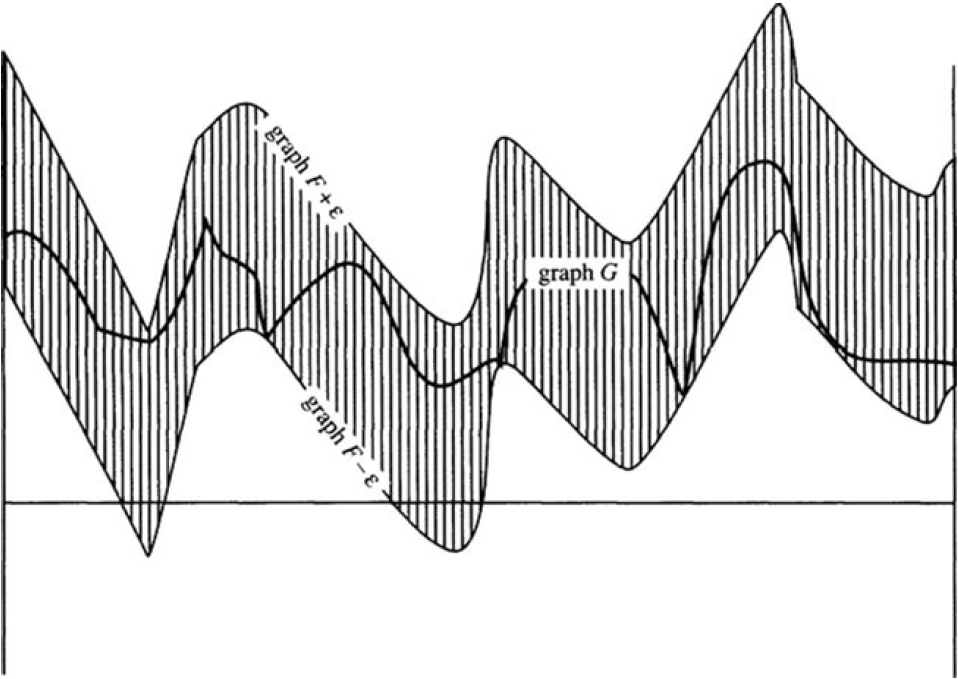
\includegraphics[width=\textwidth]{images/stone-weierstrass-step4.png}}
        \end{column}
    \end{columns}
\end{frame}

\section*{Anwendungen von Stone-Weierstraß}

\begin{frame}
    \begin{satz}
        Jede \(2\pi\)-periodische stetige Funktion kann gleichmäßig durch ein trigonometrisches Polynom 
        \[ T(x) = a_0 + \sum_{k=1}^n a_k \cos(kx) + \sum_{k=1}^n b_k \sin(kx) \]
        approximiert werden.
    \end{satz}
    \pause
    Beweis:
    \( [0,2\pi) \) parametrisiert den Einheitskreis \(S^1\) durch \( x \mapsto (\cos x, \sin x) \). 
    \pause
    \(S^1\) ist kompakt und jede \(2\pi\)-periodische Funktion auf \(\R\) wird hier zu einer 
    stetigen Funktion auf \(S^1\).
    \pause

    Die trigonometrischen Polynome bilden eine Funktionenalgebra \( \mathcal{T} \subset \C(S^1) \), 
    die \textit{nirgends verschwindet} und \textit{Punkte trennt}.
    \pause

    Nach dem Satz von Stone-Weierstraß liegt \( \mathcal{T} \) dicht in \( \C(S^1) \). \qed
\end{frame}

\newcommand{\B}{\overline{B_1(0)}}

\begin{frame}{Vektorfelder}
    Betrachten wir ein stetiges Vektorfeld 
    \( \abb{F}{\B}{\R^2} \).\pause

    Wir wollen \( F \) durch ein Vektorfeld, das maximal endlich 
    häufig verschwindet, approximieren.
    \pause

    Betrachte die Funktionenalgebra \( \A \subset \C(\B) \) 
    der reellen Polynome in zwei Variablen \pause
    \[ \A = \set{ x \mapsto \sum_{i,j=0}^n c_{ij} x^i y^j \;|\; c_{ij} \in \R }. \]
    \pause

    Dies ist eine Algebra, die \textit{nirgends verschwindet} und \textit{Punkte trennt}.
    \pause

    Aus dem Satz von Stone-Weierstraß folgt, dass \(A\) dicht in \( \C(\B) \) ist 
    und so können wir \( F = (F_1, F_2) \) durch Polynome 
    \( F_1 \approx P, F_2 \approx Q \) approximieren.
\end{frame}